\documentclass[conference]{IEEEtran}
\IEEEoverridecommandlockouts
% The preceding line is only needed to identify funding in the first footnote. If that is unneeded, please comment it out.
\usepackage{cite}
\usepackage{amsmath,amssymb,amsfonts}
\usepackage{algorithmic}
\usepackage{graphicx}
\usepackage{textcomp}
\usepackage[table,xcdraw,dvipsnames]{xcolor}
\usepackage{hyperref}
\usepackage{bookmark}
\usepackage{tabularx}
\usepackage{array}
\usepackage{colortbl}
\usepackage{etoolbox}

\newcommand{\TODO}[1]{\textbf{TODO (#1): }}

\def\BibTeX{{\rm B\kern-.05em{\sc i\kern-.025em b}\kern-.08em
    T\kern-.1667em\lower.7ex\hbox{E}\kern-.125emX}}
\graphicspath{ {./images/} }


\begin{document}

\title{Presentable Debugging with LLVManim}
\thispagestyle{plain}
\pagestyle{plain}

\author{\IEEEauthorblockN{Benjamin Houle}
\IEEEauthorblockA{\textit{Dept. of Computer Science} \\
\textit{University of Massachusetts Lowell}\\
Lowell, Massachusetts, USA \\
Benjamin\_Houle@student.uml.edu}
\and
\IEEEauthorblockN{Ebenezer Oloyede}
\IEEEauthorblockA{\textit{Dept. of Computer Science} \\
\textit{University of Massachusetts Lowell}\\
Lowell, Massachusetts, USA \\
Ebenezer\_Oloyede@student.uml.edu}
\and
\IEEEauthorblockN{Lily Grippo}
\IEEEauthorblockA{\textit{Dept. of Computer Science} \\
\textit{University of Massachusetts Lowell}\\
Lowell, Massachusetts, USA \\
Lily\_Grippo@student.uml.edu}
\and
\IEEEauthorblockN{Mohammad Ahmed}
\IEEEauthorblockA{\textit{Dept. of Computer Science} \\
\textit{University of Massachusetts Lowell}\\
Lowell, Massachusetts, USA \\
ahmedzubair16dec@gmail.com}
}

\maketitle

\begin{abstract}
LLVManim is a code visualization tool that generates aesthetically pleasing animations for information control flow and memory allocations. Utilizing the well-supported Manim library alongside LLVM’s built-in static analysis tools and wide language support, LLVManim is able to quickly create informative, professionally styled animations for any code that compiles to LLVM IR. The primary objective of the project is to create an alternative to the unappealing “programmer art” and visual clutter that many standard tools suffer from, instead focusing on an output more suitable for presentations or educational purposes.
\end{abstract}

\begin{IEEEconcepts}
Human-centered computing $\rightarrow$ Visualization $\rightarrow$ Visualization systems and tools $\rightarrow$ Visualization toolkits;
$\bullet$~Software and its engineering $\rightarrow$ Software notations and tools $\rightarrow$ Compilers;
$\bullet$~Applied computing $\rightarrow$ Education $\rightarrow$ Interactive learning environments
\end{IEEEconcepts}

\begin{IEEEkeywords}
program visualization, code animation, LLVM, static analysis, control flow graphs, memory visualization, educational tools, Manim, compiler infrastructure, presentation tools
\end{IEEEkeywords}


\section{Introduction}
Despite static analysis and data visualization being among the oldest concepts in computer science, it seems that disappointingly few graphic designers have been significantly interested in the former. While plenty of tools exist for creating control flow graphs or visualizing the stack, the majority of these favor a “function over form” paradigm that focuses on creating light-weight readable output, assuming the user is more concerned with the information than its presentation. This, however, is not always the case: presenting in any context, such as at a conference or school, generally favors quickly digestible and visually appealing content opposed to static, large blocks of text. In
these cases, the presenter is currently forced to choose between using the unappealing generated visualization and the slog of creating something presentable for themselves.

\section{Existing Tools}
\subsection{PythonTutor}
PythonTutor\cite{pythontutor} is a widely used educational tool for visualizing program execution, originally developed to help novices build accurate mental models of how code runs. Its core contribution is a step‑by‑step execution trace that exposes stack frames, heap objects, and control flow in a concrete, visual manner. As described by its creator, Philip J. Guo, PythonTutor aims to "help people overcome a fundamental barrier to learning programming: understanding what happens as the computer runs each line of code" \cite{Guo2013}.

\begin{figure}[htbp]
\centerline{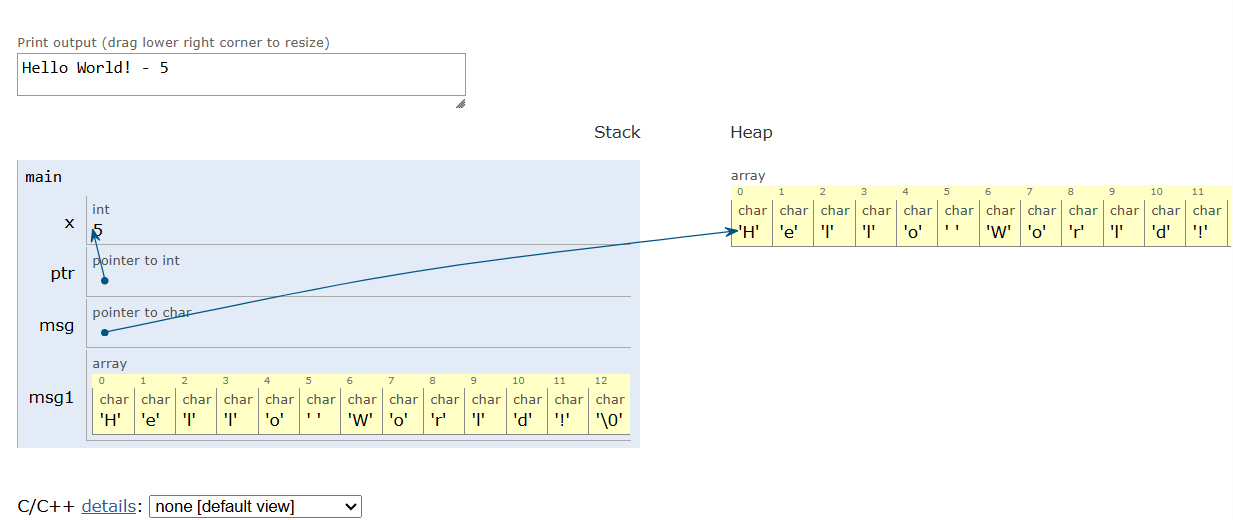
\includegraphics[width=\linewidth]{PythonTutor.PNG}}
\caption{Example Pythontutor.com output.}
\label{fig:pythontutor}
\end{figure}

In fact, PythonTutor has been shown to be effective in improving students' understanding of programming concepts; Guo's further studies demonstrated significant learning gains when PythonTutor was used as a supplement to traditional instruction \cite{Guo2015}. This shows the educational value of connecting code execution to visual representations, as well as the benefits of an accessible, interactive
tool.

However, the visualizations produced by PythonTutor are relatively basic and not suitable for presentation purposes. PythonTutor's primary focus is on clarity and educational value rather than aesthetics, resulting in output that may be difficult to read or visually unappealing when projected to an audience. This, along with the fact that the tool is web-based and not designed for offline use, makes it less than ideal for use in settings such as conference presentations where visual impact is important. PythonTutor is additionally restricted by its limited customization options, minimal library of visualization methods, and support for only C, C\thinspace\verb|++|, Java, Javascript, and Python.

\subsection{LLVM Analysis and Transform Passes}
LLVM has emerged as the de-facto standard compiler infrastructure for modern software development, powering everything from the development environment for Apple operating systems to cutting-edge systems research efforts. Its adoption by the compiler community can be attributed to several key strengths--a modular architecture that separates language frontends from optimization backends, an extensive suite of analysis and transformation passes that expose deep insights into program behavior, and robust support for numerous programming languages including C, C++, Rust, Swift, and Julia \cite{LLVM2004}.

At the core of LLVM's value proposition for code analysis is its Intermediate Representation (IR), a low-level and platform-independent format that captures program semantics in a standardized way. This IR serves as the foundation for powerful built-in analysis passes that can generate control flow graphs, dominator trees, data flow analyses, and detailed memory access patterns. For compiler developers and researchers, these capabilities are invaluable—LLVM effectively solves the hard problem of extracting structured information from code, allowing them to focus on higher-level tasks like optimization or verification \cite{LLVMRef}.

However, LLVM's visualization capabilities tell a different story. The standard approach for visualizing analysis results relies on generating DOT\footnote{Abstract grammar for defining Graphviz nodes, edges, graphs, subgraphs, and clusters.} files through passes like \texttt{-dot-cfg} or \texttt{-view-cfg}, which are then rendered using Graphviz\cite{graphviz}. While functionally correct, the resulting diagrams embody a strictly utilitarian aesthetic: monochrome nodes and edges, densely packed labels filled with LLVM IR instructions, and layouts optimized for completeness rather than clarity. This "function over form" philosophy serves well enough as a developer tool for debugging optimizer passes, but it fails catastrophically as a solution for communication beyond that narrow domain. A lecturer explaining recursion to undergraduates, a tech lead presenting architectural decisions to stakeholders, or a researcher delivering a conference talk all face the same problem: LLVM-generated visualizations are too dense, too technical, and frankly, too ugly to serve their pedagogical or presentational needs.

\begin{figure}[htbp]
\centerline{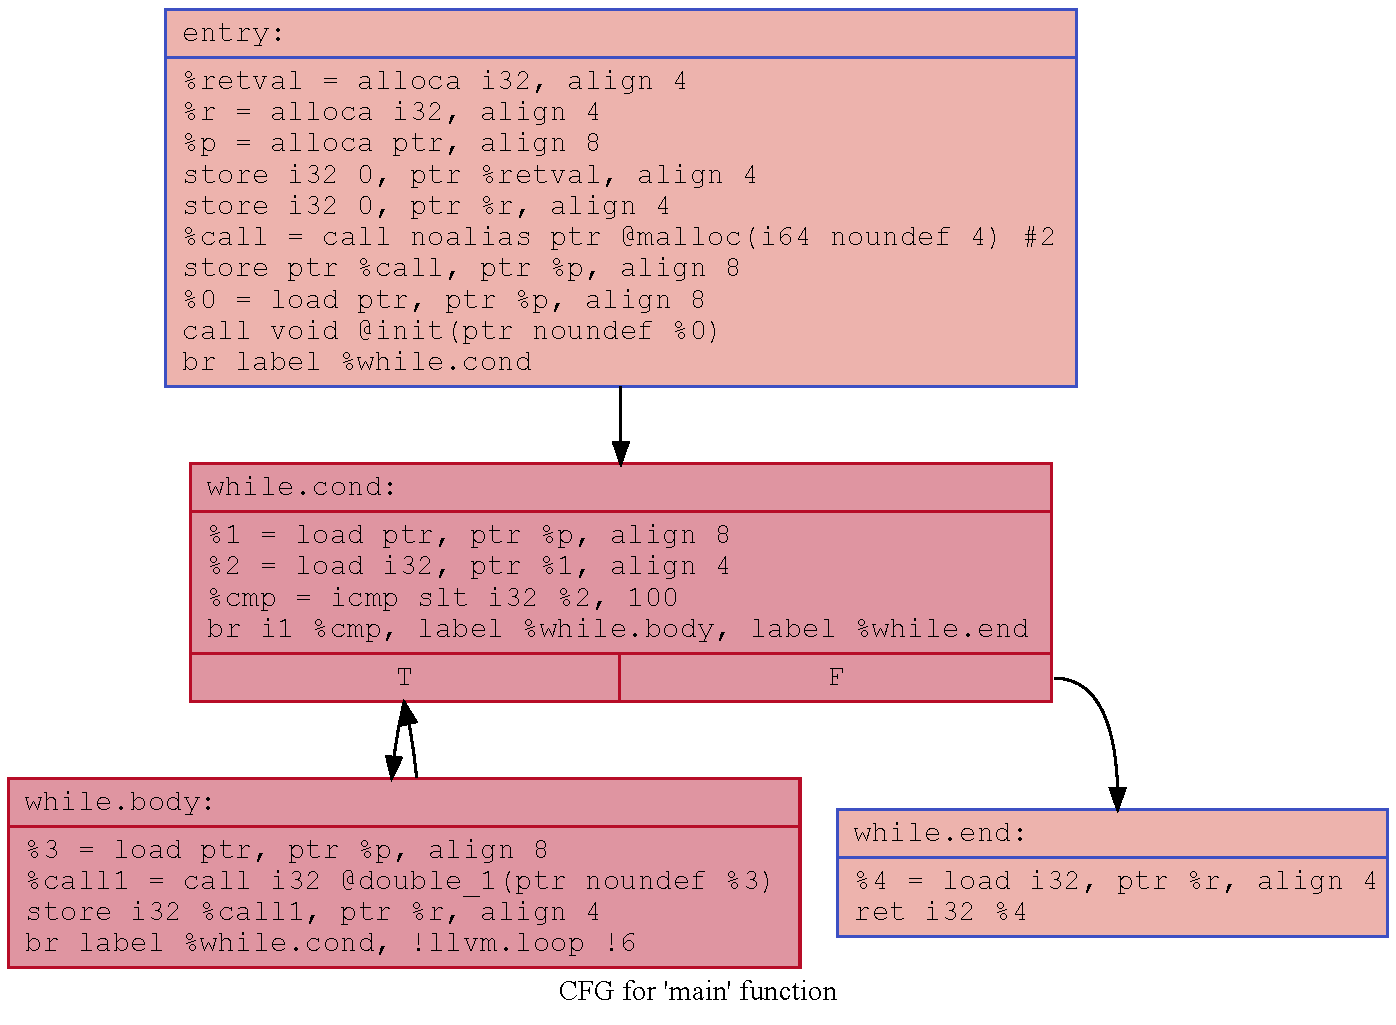
\includegraphics[width=\linewidth]{images/CFG.pdf}}
\caption{Example Control Flow Graph using LLVM \texttt{-dot-cfg} pass. While technically accurate, the visualization prioritizes information density over visual clarity.}
\label{fig:cfg}
\end{figure}

The barrier extends beyond mere aesthetics. Interpreting these diagrams requires familiarity with LLVM IR syntax—understanding what ``\texttt{\%4 = load i32, i32* \%3}'' means demands compiler knowledge that most audiences lack. The visualizations are fundamentally static images with no mechanism for progressive disclosure or animation, forcing presenters to mentally simulate execution flow while pointing at a frozen graph. Moreover, customization options are severely limited; changing colors, adjusting layouts, or highlighting specific execution paths requires manual post-processing in external tools, completely defeating the purpose of automated generation.

In essence, LLVM provides extraordinarily powerful analysis capabilities but pairs them with visualization tools that assume their primary consumer is someone who already understands what they're looking at. This creates a frustrating gap: we can automatically extract rich semantic information about program behavior, but we cannot automatically present that information in a way that serves educational or presentational contexts. LLVManim aims to bridge this gap by maintaining LLVM's analytical rigor while replacing its austere output with animations designed for human communication rather than machine precision.

\section{Manim}
The Manim library\cite{manim} was originally developed by Grant Sanderson\cite{3b1b-website} for his popular educational YouTube channel "3Blue1Brown" to create animations of mathematical and computer science concepts.\cite{3b1b-channel} His approachable animations have helped him become one of the most well-known online educators in these fields and have helped countless others understand complex topics more easily. Given this history, Manim represents an excellent candidate for creating high-quality educational presentations. Unfortunately, many potential users lack either the ability or the willingness to invest the substantial time required to create custom animations with this Python library.

While tools like PythonTutor and LLVM successfully address the technical challenge of extracting and displaying program information, they fall short in making that information genuinely engaging. This is where Manim distinguishes itself, not as a code analysis tool, but as a demonstration of what becomes possible when visualization prioritizes both clarity and aesthetic appeal.

Since its inception in 2015, the 3Blue1Brown channel has gained more than 6 million subscribers and hundreds of millions of views. Individual videos on topics such as linear algebra, calculus, and even neural networks regularly reach audiences of millions. Sanderson's approach, using smooth, precisely choreographed animations to build intuition about abstract concepts, has earned him widespread recognition in the educational community. The key to all of these animations is Manim, an animation engine written in Python and maintained by Sanderson himself.

Manim's strength lies in its ability to programmatically generate animations with mathematical precision. Instead of tiresome keyframe animation like other software, Manim allows users to write Python code to determine how different mathematical objects should look, change, and interact with each other. Manim can render beautiful 3D scenes, render LaTeX equations, and output crisp 60 fps animations for any purpose, from YouTube tutorials to academic conferences. What makes Manim unique for education is its capacity to make complicated ideas, like matrix transformations, function composition, or even program flow, tangible and understandable to the viewer by systematically unfolding them.

Yet, this power comes with a barrier to entry. It is not trivial for a professor who wants to make a presentation for a single lecture, or a researcher who wants to create visualizations for a conference presentation, to learn and use Manim effectively. They may have a clear idea of what they want to show, perhaps how a recursive function builds up its stack, but writing Manim code for it requires a distinct skill set. LLVManim addresses this challenge by automatically translating program semantics into visual representations, thereby eliminating the barrier of manual coding between LLVM's analytical power and Manim's visual sophistication.

\section{LLVManim}
By providing a solution to quickly and easily create data-based animations,
LLVManim aims to bridge the gap between these two concepts:
\begin{enumerate}
    \item Methods exist to quickly generate code visualizations, but they are
    unappealing for presentation purposes.
    \item The Manim library can make visually impressive animations, but using
    it is time consuming.
\end{enumerate}
Educators and tech leads alike can rejoice in spicing up their PowerPoints
without needing to compromise between style and accessibility.


\subsection{Project Goals}
The primary goal of LLVManim is to create a lightweight pipeline for converting
LLVM IR and runtime traces into concise, animated explanations of program
behavior. As a proof-of-concept, the initial version of LLVManim will focus on
visualizing fundamentals, such as control flow and memory allocations.

\textbf{Proof-of-Concept Targets:}
\begin{itemize}
    \item \textbf{IR Instruction Coverage:} Support for the most common LLVM IR
    instructions, such as \texttt{load}, \texttt{store}, \texttt{call}, and
    basic arithmetic operations. This will allow LLVManim to visualize a wide
    range of simple programs.
    \item \textbf{Trace Event Mapping:} Correctly map $\geq 95\%$ of runtime
    events (loads, stores, branches, calls, returns) to IR locations when debug
    metadata is present.
    \item \textbf{Customization Options:} Provide $\geq 4$ user-configurable
    options $-$ Analysis method, animation speed, color palette, \& verbosity.
    \item \textbf{Usability:} In a pilot study (6–8 participants), achieve
    $\geq~80\%$ task completion for locating injected bugs.
\end{itemize}

\textbf{Core Features:}
\begin{itemize}
    \item \textbf{LLVM IR Parsing:} Extract control flow and memory access
    information from LLVM IR, utilizing debug metadata when available.
    \item \textbf{Manim Animation Generation:} Translate LLVM IR and trace
    information into Manim scenes that visually represent control flow, stack
    frames, heap allocations, and data flow.
    \item \textbf{User Interface:} Develop a simple command-line
    interface that allows users to specify input files, select visualization
    options, and generate animations with minimal configuration.
    \item \textbf{Basic Animation Customization:} Allow users to customize the
    appearance of animations (e.g. color schemes, animation speed, etc.) to suit
    different presentation contexts.
    % \item \TODO{non-critical} Come up with more core features.
\end{itemize}

\textbf{Major features (required to realize the intended product):}
\begin{itemize}
    \item \textbf{Advanced Animation Customization:} Allow users to customize
    more aspects of the animations, such as layout styles, node shapes, or
    animation effects.
    \item \textbf{Basic Interactive Features:} Implement basic interactivity in
    the generated animations, such as pausing, stepping through execution, or
    highlighting specific paths.
    % \item \TODO{non-critical} Come up with more major features.
\end{itemize}

\textbf{Stretch features (nice‑to‑have if time permits):}
\begin{itemize}
    \item \textbf{GUI:} Create a graphical user interface for users who prefer
    not to use the command line.
    \item \textbf{Advanced Interactive Features:} Implement advanced
    interactivity in the generated animations, such as allowing users to click
    on nodes to see underlying IR code or variable values.
    % \item \TODO{non-critical} Come up with more stretch features.
\end{itemize}


\subsection{Implementation Plan}
We approach the implementation of LLVManim as a 3-layer architecture:
\textbf{Ingestion}, \textbf{Transformation}, and \textbf{Presentation}. The
Ingestion layer collects LLVM IR and metadata. The transformation layer maps the
collected IR constructs and trace events to an intermediate scene graph. The
presentation layer renders the scene graph with Manim animations and exposes a
small API for interactive playback.

\begin{figure}[htbp]
\centerline{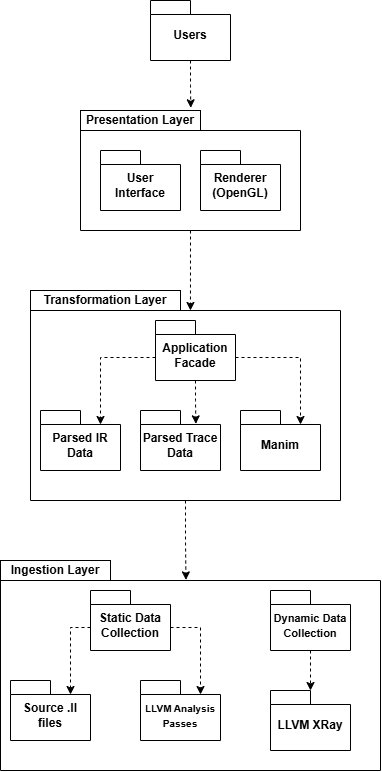
\includegraphics[width=\linewidth]{Model_Diagram}}
\caption{Model diagram illustrating the three-layer architecture of LLVManim. The Ingestion layer collects LLVM IR and metadata, the Transformation layer maps it to an intermediate scene graph, and the Presentation layer renders it with Manim animations.}
\label{fig:model_diagram}
\end{figure}

\subsubsection{User Interface}
Command-line interface with automatic compilation:

{\small
\begin{verbatim}
# Visualize C program
llvmanim factorial.c --mode cfg 
    --output demo.mp4

# Custom speed and colors
llvmanim quicksort.c --mode memory 
    --speed 0.75 --palette dark 
    --output sort.mp4

# Interactive mode
llvmanim recursive.c --mode trace 
    --interactive
\end{verbatim}
}

\subsubsection{Presentation Layer}
The Presentation layer renders the scene graph using Manim.

Key operations:
\begin{itemize}
    \item \textbf{Manim Code Generation:} Translate scene graph into Python code defining a Manim \texttt{Scene} class. Visual elements become \texttt{Mobject} instances with animation commands.
    \item \textbf{Rendering Pipeline:} Invoke Manim to produce MP4 video or enable interactive preview with keyboard controls.
    \item \textbf{Customization API:} Provide configuration options using command line flags and YAML files:
    \begin{itemize}
        \item \texttt{--speed <factor>}: Animation playback speed
        \item \texttt{--palette <name>}: Color scheme (dark, light, colorblind)
        \item \texttt{--mode <type>}: Visualization mode (cfg, memory, trace)
        \item \texttt{--verbose}: Include IR instruction text
    \end{itemize}
\end{itemize}

\subsubsection{Transformation Layer}
The Transformation layer maps LLVM constructs to an intermediate scene graph for Manim rendering.

Key operations:
\begin{itemize}
    \item \textbf{Scene Graph Construction:} Create hierarchical representation where nodes correspond to visual elements (basic blocks, stack frames, memory cells) with properties for position, appearance, and timing.
    \item \textbf{Layout Algorithm:} Apply hierarchical layout to position CFG nodes while minimizing edge crossings and maintaining logical flow direction. We use a modified Sugiyama framework with constraints for common patterns like if-else branches and loop back-edges.
    \item \textbf{Instruction-to-Animation Mapping:} Define animation primitives for each LLVM instruction:
    \begin{itemize}
        \item \texttt{alloca}: Create stack frame with variable label
        \item \texttt{load}/\texttt{store}: Animate arrow to/from memory location
        \item \texttt{call}: Push new stack frame with fade-in
        \item \texttt{ret}: Pop stack frame with fade-out
        \item \texttt{br}: Highlight control flow edge with color change
    \end{itemize}
    \item \textbf{Timing Coordination:} Calculate timing offsets for animation events (default 1 second per instruction, user-configurable).
\end{itemize}

\subsubsection{Ingestion Layer}
The Ingestion layer extracts program structure from LLVM IR. We use the \texttt{llvmlite} Python binding to parse .ll files generated by clang with the \texttt{-g} flag for debug metadata.

Key operations:
\begin{itemize}
    \item \textbf{IR Parsing:} Load LLVM modules and extract functions, basic blocks, and instructions.
    \item \textbf{Control Flow Extraction:} Build CFGs by analyzing branch instructions and identifying successor relationships between blocks.
    \item \textbf{Metadata Collection:} Extract debug information like source line numbers, variable names, and types from LLVM debug intrinsics.
    \item \textbf{Memory Operation Identification:} Catalog memory-related instructions including \texttt{load}, \texttt{store}, \texttt{alloca}, and \texttt{call} for tracking memory access patterns and stack operations.
    \item \textbf{Output:} Structured representation with CFG, instruction list, and metadata stored in Python dictionaries mapping basic block IDs to instruction sequences.
\end{itemize}

The tool compiles .c/.cpp files to LLVM IR automatically or processes .ll files directly. Error messages indicate unsupported features with workarounds.


\section{Projected Timeline}

% Please add the following required packages to your document preamble:
% \usepackage{graphicx}
% \usepackage[table,xcdraw]{xcolor}
% Beamer presentation requires \usepackage{colortbl} instead of \usepackage[table,xcdraw]{xcolor}
\begin{table}[htbp]
\centering
\renewcommand{\arraystretch}{1.5}
\rowcolors{2}{white}{gray!20}
\begin{tabularx}{\columnwidth}{|>{\centering\arraybackslash}m{2.5cm}|>{\raggedright\arraybackslash}X|}
\hline
\rowcolor[HTML]{4472C4}
\textcolor{white}{\textbf{Week}} & \textcolor{white}{\textbf{Task}} \\ \hline
$W_1$    [$2/08 - 2/14$] & $\bullet$ Project proposal draft complete.\newline
                           $\bullet$ Development environment setup. \\ \hline
$W_2$    [$2/15 - 2/21$] & $\bullet$ LLVM Parsing \\ \hline
$W_3$    [$2/22 - 2/28$] & $\bullet$ Stack Frame Animation \\ \hline
$W_4$    [$3/01 - 3/07$] & $\bullet$ Heap Animation \\ \hline
$W_5$    [$3/08 - 3/14$] & $\bullet$ User Interface\\ \hline
$W_6$    [$3/15 - 3/21$] & $\bullet$ Interactive feature: Step,Pause \\ \hline
$W_7$    [$3/22 - 3/28$] & $\bullet$ Animation Speed and Color \\ \hline
$W_8$    [$3/29 - 4/04$] & $\bullet$ Code Testing \\ \hline
$W_9$    [$4/04 - 4/10$] & $\bullet$ Code Testing\\ \hline
$W_{10}$ [$4/11 - 4/17$] & $\bullet$ Additional Feature\\ \hline
\end{tabularx}
\vspace{0.1cm}
\caption{Projected timeline for LLVManim Development.}
\end{table}

\section{Feedback}
\begin{quotation} [1]
"The figures are helpful for showing how the existing tools work, but for the
proposal make sure you show how you want the visualized code to work.  This
could be through making a mockup or setting up input for Manim to generate
something that looks like what you want.  You should also think about the
pipeline for what data you are planning on getting from LLVM, how you are going
to get it, and how you will feed it into Manim."
\end{quotation}

\noindent This feedback remains unaddressed at present, primarily due to time constraints during the proposal development phase. We intend to create a mockup of the intended output in the near future to better illustrate our vision for the final product.

\begin{quotation} [2]
  "You have figures for some existing tools.  Make sure you talk about them in the proposal and what their limitations are."
\end{quotation}

\noindent\hrulefill

\begin{quotation} [3]
  "This [PythonTutor] figure is unreadable."
\end{quotation}

\begin{quotation} [4]
  "[PythonTutor] Spelling"
\end{quotation}

\begin{quotation} [5]
  "Which languages [are supported by PythonTutor]?"
\end{quotation}

\begin{quotation} [6]
  "You should have a citation for where to access the [PythonTutor] tool itself and not just the paper describing its efficacy."
\end{quotation}

\begin{quotation} [7]
  "The text in the [control-flow graph] figure is too small."
\end{quotation}

\begin{quotation} [8]
  "[Graphviz] Linky please"
\end{quotation}

\begin{quotation} [9]
  "Linky to Manim."
\end{quotation}

\begin{quotation} [10]
  "citation needed [for 3Blue1Brown's winning a Streamy award]"
\end{quotation}

\begin{quotation} [11]
  "The order of the [model] diagram is in the opposite order that they are presented in [implementation plan] text."
\end{quotation}

\begin{quotation} [12]
  "The items in the timeline are incredibly brief and need more detail or support."
\end{quotation}

\noindent\hrulefill

\begin{quotation} [13]
  "The figures are quite shrunk down especially figure 1 and figure 2 making it extremely difficult to read the content within it, if those were made larger it would greatly improve the readability."
\end{quotation}

\begin{quotation} [14]
  "The abstract clearly explains the purpose and motivation of LLVManim, especially its goal of improving visualization aesthetics for presentations and education. However, it could briefly mention the intended users explicitly, such as educators, students, or software engineers. Additionally, the abstract could briefly summarize how LLVManim achieves this goal rather than only stating the objective."
\end{quotation}

\begin{quotation} [15]
  "The introduction provides strong motivation and clearly explains the gap between current visualization tools and presentation-quality output. The problem statement is well articulated, especially the distinction between “function over form” tools and presentation needs. However, the introduction could more explicitly define the scope of the LLVManim system itself earlier in the section. Currently, LLVManim is only briefly mentioned at the end. Introducing LLVManim sooner would improve clarity and help frame the remainder of the document."
\end{quotation}

\begin{quotation} [16]
  "[The PythonTutor] section clearly explains PythonTutor’s strengths and limitations. The educational benefits and usability are well supported by references, which strengthens the argument. However, this section could be slightly condensed. Some explanations regarding educational benefits are repeated, and the limitations relevant specifically to LLVManim’s goals like their lack of customization, presentation-quality output, etc., should be emphasized more clearly. Additionally, explicitly comparing PythonTutor directly to LLVManim in one or two sentences would make the relevance stronger."
\end{quotation}

\begin{quotation} [17]
  "[The LLVM Analysis and Transform Passes] section provides an excellent explanation of LLVM’s capabilities and limitations. The explanation of LLVM IR, analysis passes, and DOT visualizations is clear and technically accurate. However, this section could be improved by separating the strengths and weaknesses into clearly defined subsections or paragraphs. Currently, strengths and limitations are interwoven, which makes it slightly harder to skim. Additionally, some technical explanations like the IR syntax examples could be shortened slightly, as the focus of the proposal is visualization rather than compiler internals."
\end{quotation}

\begin{quotation} [18]
  "[The Manim] section provides an excellent explanation of Manim’s capabilities and its usefulness for creating high-quality educational animations. The explanation of its role in improving visualization aesthetics is clear and well justified. However, this section could more explicitly explain how Manim integrates into the LLVManim system pipeline. Additionally, some historical background about 3Blue1Brown could be slightly condensed to maintain focus on the project itself."
\end{quotation}

\begin{quotation} [19]
  "[The Goals and Features] section clearly defines the goals, proof-of-concept targets, and feature breakdown. The separation into proof-of-concept targets, core features, major features, and stretch features is well organized and easy to follow. However, some proof-of-concept metrics (such as $\geq95\%$ trace mapping and $\geq80\%$ usability success rate) could briefly explain how these metrics will be measured or evaluated. This would strengthen the feasibility and evaluation clarity. Additionally, the distinction between core features and major features could be clarified slightly, as both appear required for the full system."
\end{quotation}

\begin{quotation} [20]
  "[The Architecture] section provides an excellent high-level architectural overview using the three-layer model (Ingestion, Transformation, Presentation). The layered design is clear, logical, and appropriate for the system. However, the architecture diagram should be explicitly referenced and described more clearly in the text. Explaining what each arrow and component represents would improve clarity. Additionally, some implementation details (such as exact timing offsets and layout algorithms) may be overly detailed for a proposal and could be slightly condensed."
\end{quotation}

\begin{quotation} [21]
  "[The Ingestion Layer] section clearly explains how LLVM IR is parsed and structured. The use of llvmlite and debug metadata is appropriate and well explained. However, the output format could be explained more clearly, particularly how it connects to the Transformation layer."
\end{quotation}

\begin{quotation} [22]
  "The transformation layer is well explained and provides a clear mapping between LLVM constructs and animation objects. However, the scene graph structure could benefit from a brief visual example or mock representation to clarify how data flows through the system. Additionally, the modified Sugiyama layout algorithm is mentioned but not briefly explained, which may confuse readers unfamiliar with graph layout techniques."
\end{quotation}

\begin{quotation} [23]
  "[The Presentation Layer] section clearly explains how Manim is used to render animations from the scene graph. The customization options and rendering pipeline are well described. However, the relationship between scene graph generation and Manim output could be explained more clearly in terms of data flow. Additionally, it could briefly explain expected output formats and user workflows."
\end{quotation}

\begin{quotation} [24]
  "The command-line interface examples are very helpful and clearly demonstrate usability. However, this section could briefly explain error handling and limitations more clearly, such as unsupported language features or missing debug metadata. Additionally, this section could clarify whether the CLI is intended for developers, educators, or both."
\end{quotation}

\begin{quotation} [25]
  "The projected timeline is clear and logically structured. The weekly milestones align well with the system architecture and development process. However, testing and validation phases could be more clearly defined, particularly usability testing and feature validation. Additionally, stretch feature implementation is only briefly mentioned and could be explicitly identified in the timeline."
\end{quotation}

\begin{quotation} [26]
  "The feedback section properly acknowledges prior feedback and clearly states what remains unaddressed. However, this section could be improved by explicitly explaining how each feedback item will be addressed moving forward rather than only stating that it remains unaddressed. Additionally, creating mockups or example animation output would significantly strengthen the proposal and demonstrate feasibility."
\end{quotation}

\begin{quotation} [27]
  "The references are properly formatted and relevant to the proposal. The use of academic sources and official LLVM documentation strengthens credibility. However, ensure consistent formatting across all references and verify citation formatting matches IEEE or required course format exactly."
\end{quotation}

\noindent\hrulefill

\begin{quotation} [28]
  "It's unnecessary to explain how Julia works. It distracts from the main focus of the paper."
\end{quotation}

\begin{quotation} [29]
  "You don't have to include all these accomplishments. We already get the idea that [3Blue1Brown] is popular and well respected from earlier."
\end{quotation}

\begin{quotation} [30]
  "Including pictures of Manim diagrams here would illustrate your point better."
\end{quotation}

\begin{quotation} [31]
  "Your goals seem overly ambitious for just a one semester student project."
\end{quotation}

\begin{quotation} [32]
  "It's unrealistic to expect work to be done over spring break."
\end{quotation}

\begin{quotation} [33]
  "You should talk more about the potential risks. It's not really mentioned at all."
\end{quotation}

\begin{quotation} [34]
  "The motivation section could be strengthened. While the proposal explains that existing tools are either too technical or not presentation-friendly, it does not fully explain why this problem is important at a broader level. It would help to more clearly identify who specifically benefits from this tool and why current alternatives are insufficient. The proposal currently reads as though the improvement is mostly aesthetic, so emphasizing the educational or practical impact would make the motivation more compelling."
\end{quotation}

\begin{quotation} [35]
  "The objectives are generally clear, but some could be more measurable. For example, the proposal mentions performance and trace mapping goals, but it would be helpful to specify what constitutes success more concretely. Adding clearer success criteria would make it easier to evaluate whether the project meets its goals."
\end{quotation}

\begin{quotation} [36]
  "The architectural breakdown into ingestion, transformation, and presentation layers is well structured and shows strong planning. However, the scope could be clarified further. It would be helpful to specify what subset of LLVM IR will be fully supported and how unsupported constructs will be handled. Addressing potential edge cases would make the approach feel more complete and realistic."
\end{quotation}

\begin{quotation} [37]
  "The proposal would benefit from a clearer description of final deliverables. While features are described, it is not entirely clear what concrete artifacts will be submitted at the end of the project. Explicitly listing tangible deliverables would strengthen this section."
\end{quotation}

\begin{quotation} [38]
  "The timeline is present but somewhat broad in places. Some weekly goals are described generally, which makes it difficult to determine what measurable progress will be achieved each week. Making each milestone more concrete and demonstrable would better align with the rubric’s expectations.
\end{quotation}

\begin{quotation} [39]
  "The proposal mentions evaluation goals such as trace mapping percentages and usability testing, which is good. However, the evaluation methodology could be described in more detail. For example, specifying the number of participants in the pilot study, the types of tasks they will perform, and how results will be measured would make the evaluation plan stronger and more rigorous."
\end{quotation}

\begin{quotation} [40]
  "A clearly labeled risks section would improve the proposal. While potential challenges are implied, explicitly identifying technical and timeline risks and describing mitigation strategies would demonstrate thoughtful project planning."
\end{quotation}

\noindent\hrulefill

\begin{quotation} [41]
  "I feel [the PythonTutor section] should include the supported languages of PythonTutor, since the usefulness of the tool depends heavily on what languages are supported. It is more useful if it supports languages that are commonly used for education vs if it supports languages that are more obscure."
\end{quotation}

\begin{quotation} [42]
  "What are DOT files? does this mean unix dot files, or does this stand for something"
\end{quotation}

\begin{quotation} [43]
  "What does verbosity mean in this application and how is it different from animation speed. Does the creator of the animation include an audio track, or is it the speed that words appear? If the latter, how and why are words appearing?"
\end{quotation}

\begin{quotation} [44]
  "Go more in depth about what the study entails. Will you be comparing against other similar tools, or just compared to only reading the code? Will it be between subjects or within subjects? Are you only going to collect data about accuracy or will you also collect data about subjective user preference?
  
  Also this study does not seem like it connects well to the stated goal of this project. You are discussing making a tool that will help educational scenarios, but are only evaluating it for use in debugging. I would add a component focusing on user experience generating the images, or evaluating which ones help people to better understand the purpose of code

  There are also no sample graphs or tables for the data that is to be collected"
\end{quotation}

\begin{quotation} [45]
  "Why separate core features from MVP features when core features are defined as "required to have a usable product at all", which is essentially the MVP"
\end{quotation}

\begin{quotation} [47]
  "How are animations utilized. Is it moving arrows to demonstrate code flow? Will sections of the code be moved on screen only when relevant, and removed afterward. For someone unfamiliar with Manim this is unclear"
\end{quotation}

\begin{quotation} [48]
  "While I understand that this document is written with the assumption that the reader has a computer science bachelors degree, I think it would help to use the long form of this abbreviation at least once, as was done with LLVM IR."
\end{quotation}

\begin{quotation} [49]
  "Why make your own "JSON-like" format instead of just using standard JSON. If it is for data streaming purposes, perhaps consider JSON Lines"
\end{quotation}

\begin{quotation} [50]
  "No discussion of risks or costs."
\end{quotation}

\begin{quotation} [51]
  "Timeline does not say when the experiment will be performed"
\end{quotation}

\begin{quotation} [52]
  "Missing time spent on project"
\end{quotation}

\begin{quotation} [53]
  "The lack of Manim examples or proposed examples for this project makes it difficult for someone unfamiliar with that tool to understand what this tool will produce"
\end{quotation}

% \TODO{critical} describe any feedback you did NOT take action on, with a brief justification for why (for example, if some other project related to your proposal was suggested, but it is not, this is where you would say why it was not related). Include ALL feedback you have received on the project at any point, whether from the instructor or your peers. If you have addressed every piece of feedback and made changes in response, write “We have addressed all feedback.”


\section*{Acknowledgment}

We would like to thank Dr. James Daly for his guidance, feedback, and support throughout the development of this work.


\bibliographystyle{IEEEtran}
\bibliography{references}
\vspace{2em}
\textbf{HOURS SPENT:} 20 hours

\end{document}
